\documentclass{IEEEtran} %[conference]
\IEEEoverridecommandlockouts
\usepackage{cite}
\usepackage{comment}
\usepackage{enumitem}
\usepackage{amsmath,amssymb,amsfonts}
%\usepackage{algorithmic}
\usepackage{graphicx}
\usepackage{caption}
\usepackage{subcaption}
\usepackage{textcomp}
\usepackage{xcolor}
\newenvironment{bluep}{\par\color{blue}}{\par}
\def\BibTeX{{\rm B\kern-.05em{\sc i\kern-.025em b}\kern-.08em
    T\kern-.1667em\lower.7ex\hbox{E}\kern-.125emX}}
\begin{document}

\title{Computational model for temperature in tree trunk for energy harvesting\\
%{\footnotesize \textsuperscript{*}Note: Sub-titles are not captured in Xplore and should not be used}
%\thanks{\textcolor{red}{Identify applicable funding agency here. If none, delete this.}}
}

\author{\IEEEauthorblockN{Yajun An}
\IEEEauthorblockA{\textit{
School of Interdisciplinary Arts \& Sciences} \\
\textit{University of Washington, Tacoma}\\
Tacoma WA, USA \\
yajuna@uw.edu}
\and

\IEEEauthorblockN{Orlando Baiocchi}
\IEEEauthorblockA{\textit{School of Engineering and Technology} \\
\textit{University of Washington, Tacoma}\\
Tacoma WA, USA \\
baiocchi@uw.edu}
\and

\IEEEauthorblockN{Heather Dillon}
\IEEEauthorblockA{\textit{School of Engineering and Technology} \\
\textit{University of Washington, Tacoma}\\
Tacoma WA, USA \\
hedillon@uw.edu}
\and

\IEEEauthorblockN{Michael Hockman}
\IEEEauthorblockA{\textit{School of Engineering and Technology} \\
\textit{University of Washington, Tacoma}\\
Tacoma WA, USA \\
hockmm@uw.edu}
\and

\IEEEauthorblockN{Selina Teng}
\IEEEauthorblockA{\textit{College of Engineering} \\
\textit{University of Washington, Seattle}\\
Seattle WA, USA \\
seliteng@uw.edu}
}
\IEEEoverridecommandlockouts
\IEEEpubid{\makebox[\columnwidth]{978-1-7281-9615-2/20/\$31.00~\copyright2020 IEEE \hfill} \hspace{\columnsep}\makebox[\columnwidth]{ }}
\maketitle
\IEEEpubidadjcol
\begin{abstract}
The temperature difference in the cross section of a tree trunk, measured radially, generates voltage. This is leveraged to power thermoelectric devices for the purpose of environmental monitoring. The authors present a numerical model for the temperature differential within a tree stem. This model contributes to a proof of concept for the feasibility of using trees as an ambient power source for wireless devices.

The University of Washington Tacoma is in ongoing research cooperation with the University of Paraiba, Brazil and the University of the Azores, Portugal in the areas of Wireless Sensor Networks, Energy Harvesting, and Environmental Monitoring. This paper is part of these collaborative efforts and is related to the specific goal of deploying a network of wireless environmental sensors in the Island of Sao Miguel, Archipelago of the Azores, to monitor both the natural (volcanic) and industrial pollution, as well as monitoring the traffic of tourists on the island.
\end{abstract}

\begin{IEEEkeywords}
Heat Equation, Thermoelectric Generator (TEG), Computational Solutions, Numerical Model, Trees, Energy Harvesting
\end{IEEEkeywords}

\section{Introduction}
UNESCO, as part of its Geopark program, protects the Archipelago of the Azores, where the constant influx of tourists in recent years endangers the ecosystem through the pollution of the environment and the damage of protected areas. Numerical data is needed to inform policy makers about the severity of the environmental impact of tourism. Hence, the authors and collaborators at the University of the Azores (whose campus is located on the Island of Sao Miguel in the Archipelago of the Azores) propose a wireless sensor network to perform environmental monitoring  in Sao Miguel. In the current phase of the project, we built a similar experiment in the Pierce County area in Washington State. The considerations are fundamentally the same, but the latitude in Washington requires us to investigate temperature distribution in tree trunks along difference directions, whereas directions can be treated as the same in the equatorial Azores.

%We currently are working on building similar networks in forests of Washington State. The difference of the geographical locations of Washington and Azores would also have different impacts on our projects, for example, the directions at which we install devices. This requires us to investigate the temperature distribution in tree trunks along different directions. %\textcolor{red}{Ask Orlando-should we specify Washington? }

The deployment of sensor networks in remote natural areas is a challenge regarding the energy requirements of the sensors themselves and the transmission systems. Since the use of batteries is both inconvenient and environmentally unfriendly, alternative processes have been considered. In particular, energy harvesting from trees is a potential candidate.

%\subsection{Theory}
Healthy trees maintain a temperature of approximately 21.4 degrees Celsius in the leaves as a precondition for photosynthesis \ref{treeleaf}. In order to thermoregulate, the tree stores a substantial amount of heat in its stem or trunk. The annual rings in a tree trunk (Fig. 1) can thus be treated as isothermal sub-volumes. Reference \ref{souza} asserts that the temperature gradient between any annual ring and the external temperature is either approximately constant or varies with some time-delay as the external temperature varies. 

In order to utilize the small amount of energy obtained from the trees, it is important to know the heat distribution inside the trees as a function of the nature of the trees, the solar radiation, and the specific characteristics of the environment in which the harvesting takes place. That is the purpose of this paper, which uses mathematical modeling and simulation of the conversion of heat into electricity via the Seebeck effect. 

%\begin{figure}
%  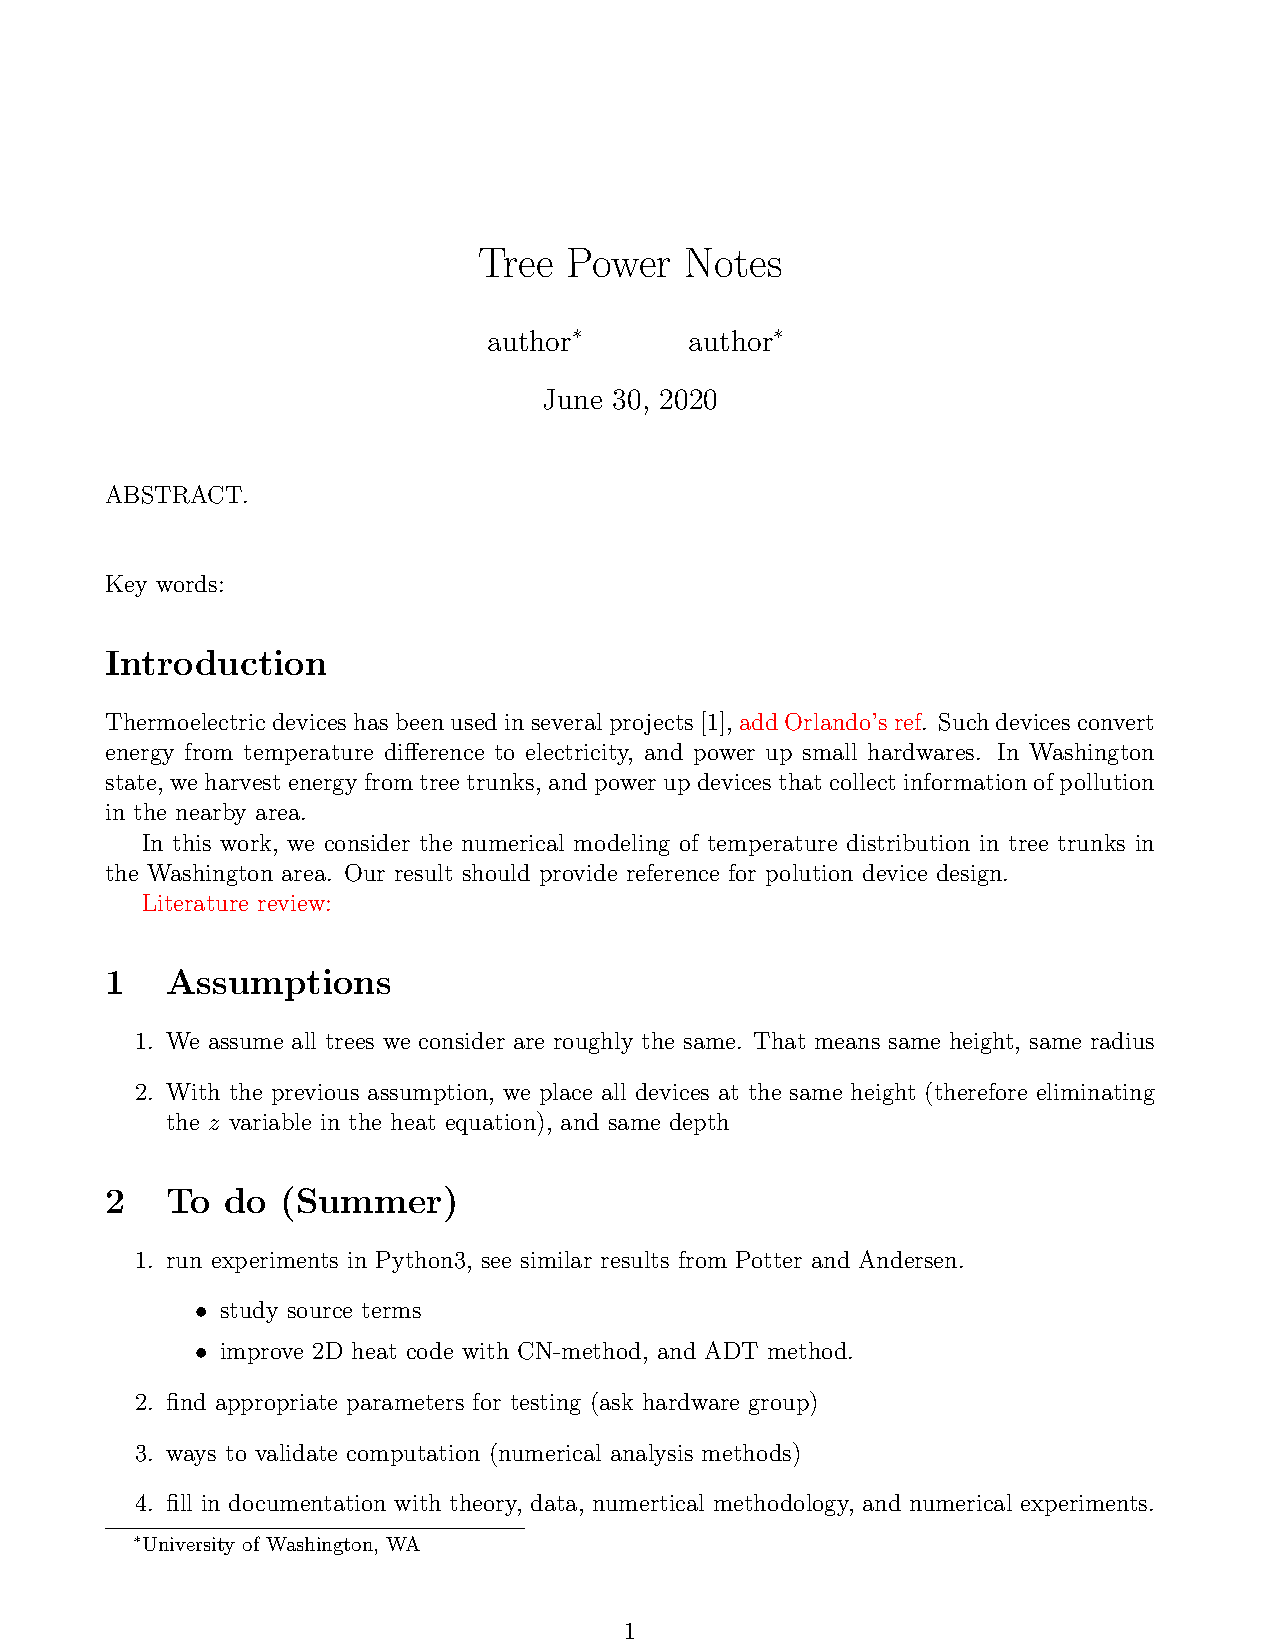
\includegraphics[width=1\linewidth]{fig/tree.jpg}
%  \caption{Tree Stem Cross Section. Source: \ref{souza}}
%  \label{fig:tree_diagram}
%\end{figure}

To harvest the energy, we use a thermoelectric generator attached to a metal rod, which is driven laterally through the tree stem. Although they are less efficient than heat engines, thermoelectric generators (TEGs) are preferred in remote applications that only require low power, which suits the relatively low output expected from natural heat sources such as trees \ref{souza}. The use of tree stems as a heat source for TEGs is promising because it is a long-lasting, maintenance-free energy source, suitable for powering local wireless devices, such as environmental sensors. Our group hypothesizes that the most crucial element of the TEG system is the way in which the temperature of the interior of the tree is brought into contact with the TEG.


%\begin{figure}
%    \centering
%    \begin{minipage}{0.24\textwidth}
%        \centering
%        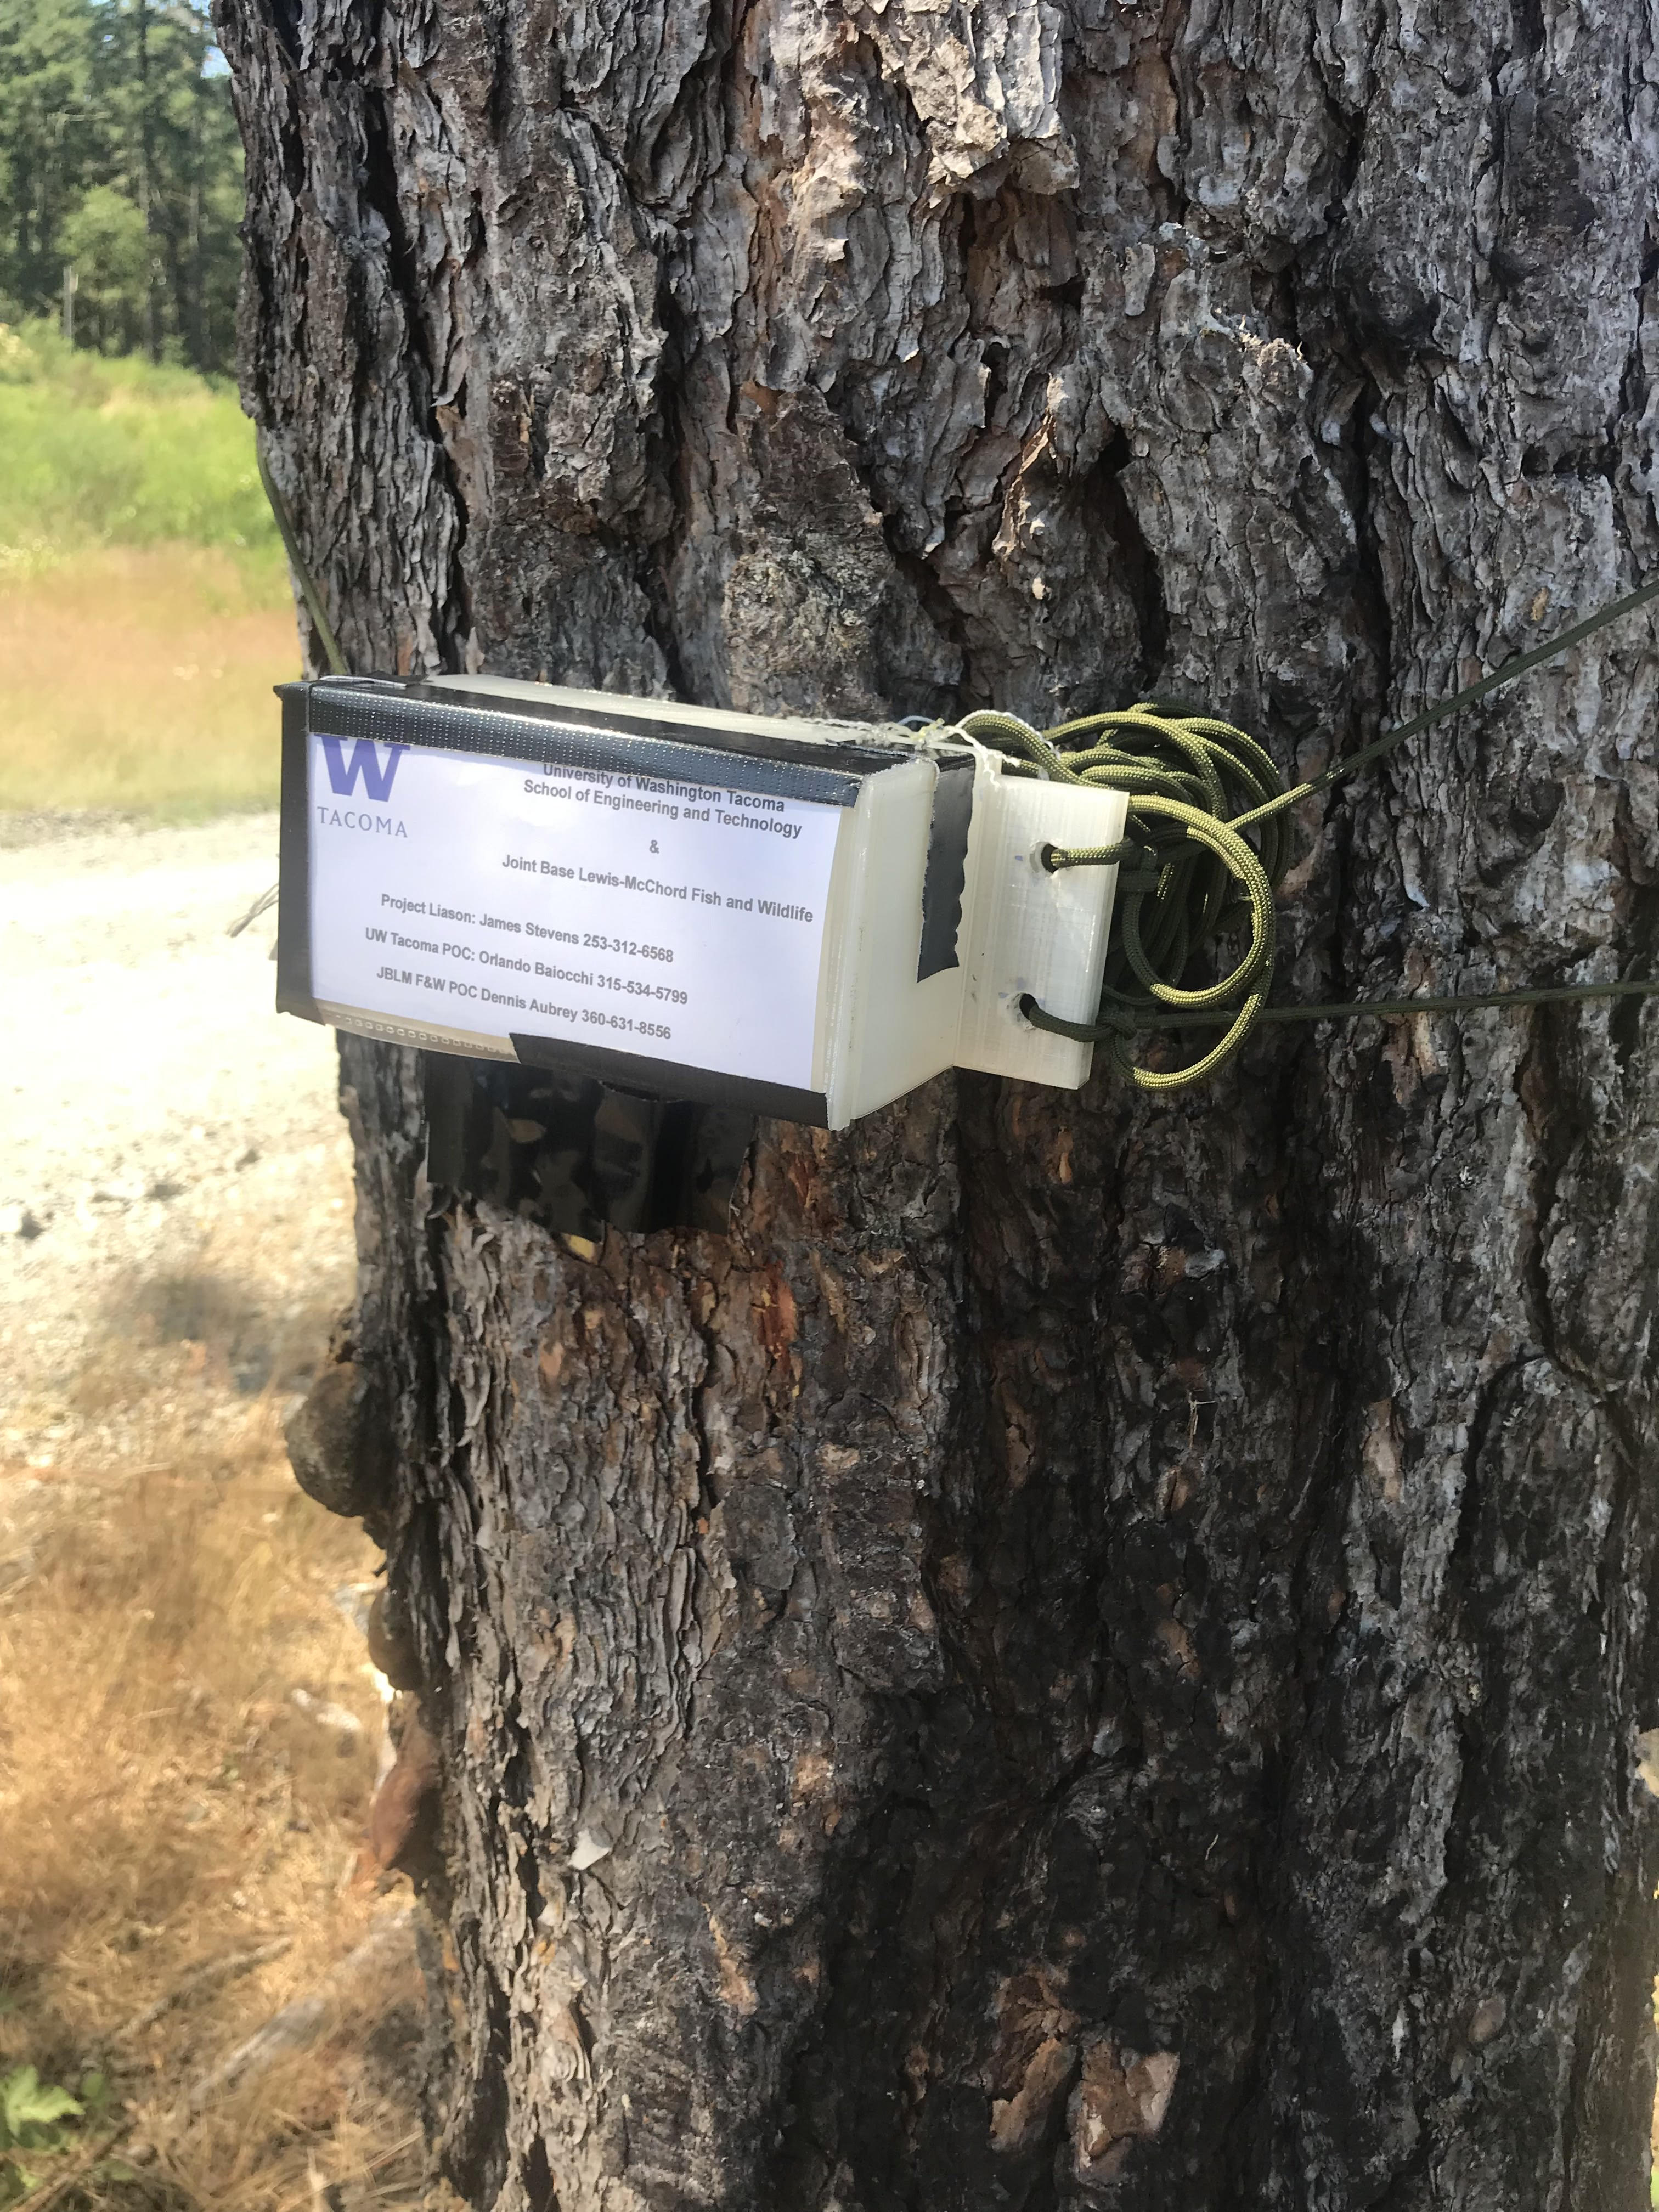
\includegraphics[width=1\textwidth]{fig/device.jpg} % first figure itself
%        %\caption{first figure}
%    \end{minipage}\hfill
%    \begin{minipage}{0.24\textwidth}
%        \centering
%        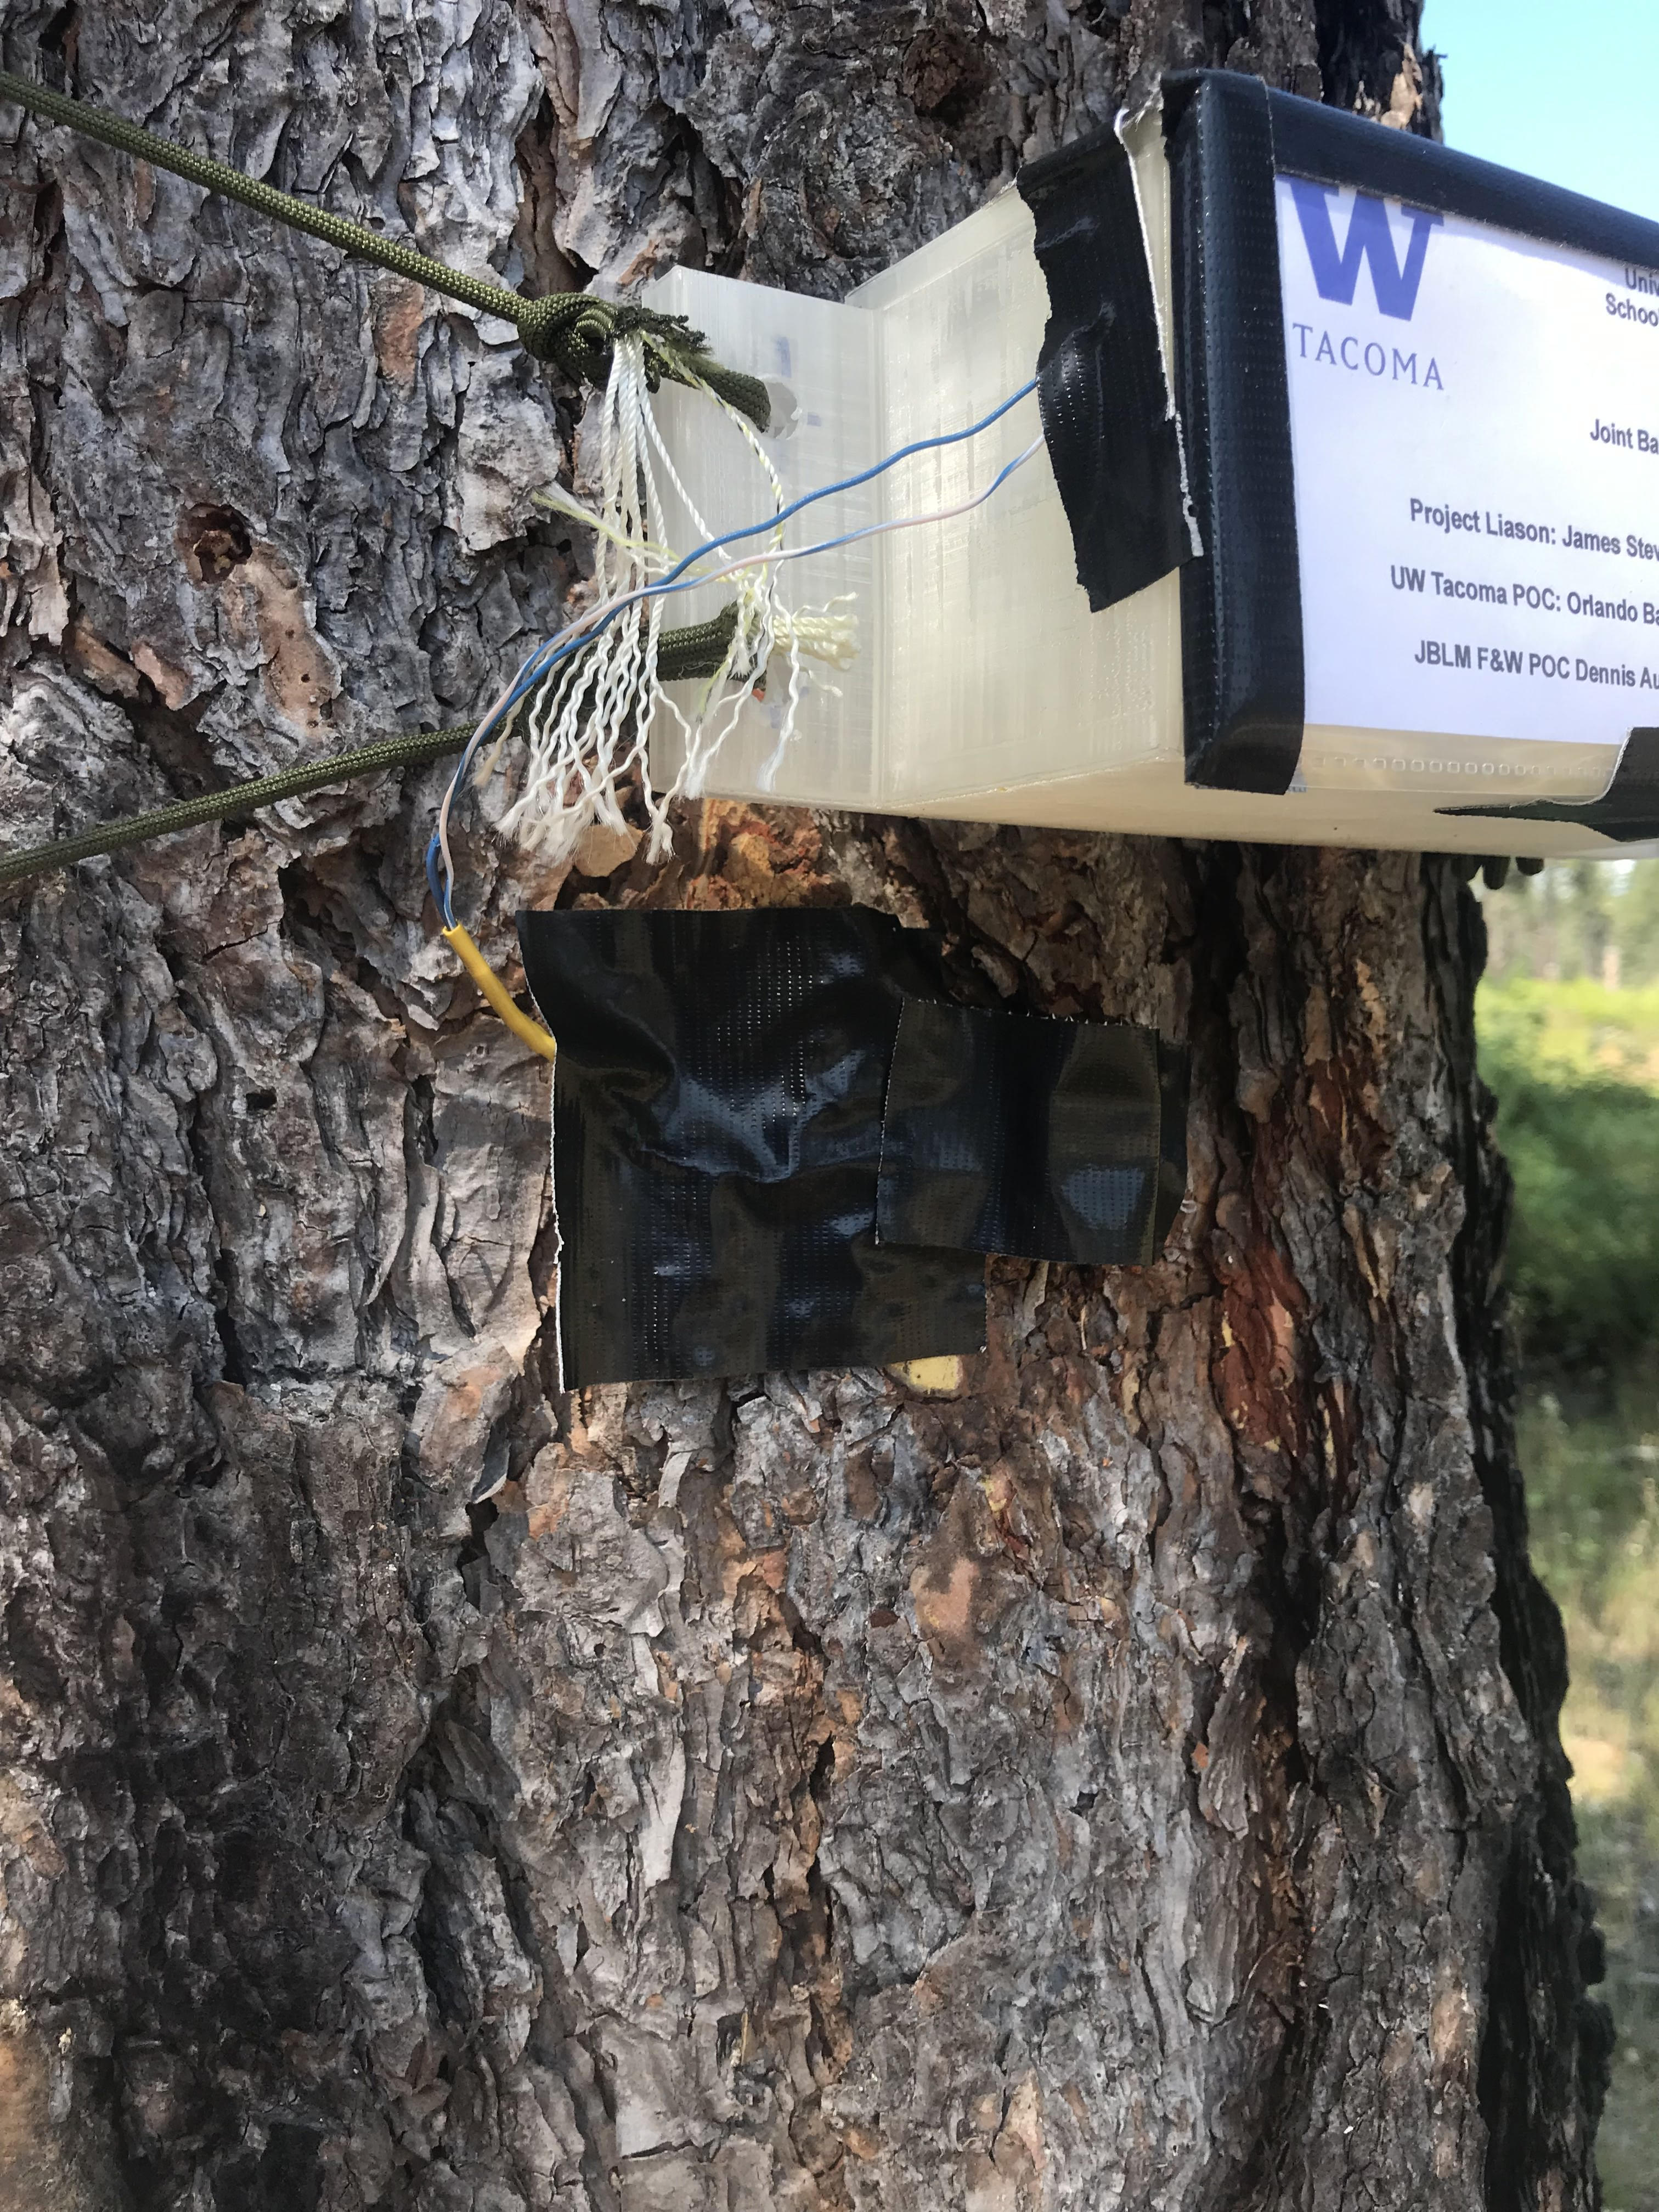
\includegraphics[width=1\textwidth]{fig/device1.jpg} % second figure itself
%        %\caption{second figure}
%    \end{minipage}
%    \caption{TEG devices installed on tree trunks in Washington State}
%    \label{fig:TEG}
%\end{figure}

In this work, we \begin{bluep}present mathematical models simulating the temperature distribution in tree trunks with partial differential equations (PDEs) and their numerical solutions, with the purpose of examining the efficacy of trees for energy harvesting. \ref{potter_andresen} presented an earlier 2D model to simulate tree temperature distributions, driven by the influences of solar radiation, infrared emission and absorption, convection, and conduction. Their numerical solutions were obtained by a Finite Difference (FD) scheme, with centered differencing in space, and leapfrog in time. Another 2D temperature distribution model for tree trunks, FireStem2D, has been created by \ref{firestem2d}. FireStem2D has parameters for studying the effects of forest fires on tree stem injury, whereas the present paper examines the temperature of trees in ambient conditions. 

The present work focuses on a simplified 1D PDE model that retains the needed sensitivity for the energy harvesting task.  In the next section, we justify the simplification obtained by reducing the dimensions from 3D to 2D, then to 1D). We follow the source terms used in Potter and Andresen model  \ref{potter_andresen}. In handling heat source, we treat the heat flux as the only source and solve a boundary value problem from the converted temperature condition. We apply a homogenous Neumann condition at the center of the tree trunk \ref{firestem2d}, and a nonhomogenous Dirichlet condition at the bark surface. We solve the differential equation in one dimension numerically using the Crank-Nicolson method, which is superior to explicit methods in its stability, thereby reducing the computation cost. 

This project is a work in progress; we present PDE models and their numerical solutions based on example data from current literature \ref{potter_andresen}, since the COVID-19 pandemic has impacted our plans to collect field data in Washington State. Our result should provide reference for hardware analysis, particularly, giving insight to the magnitude of voltage possible for the thermoelectric devices. First we describe the PDE, including the justification for dimension reduction, source terms, and example input data. We describe the implementation of the FD scheme in polar coordinates with the Crank-Nicolson method, and boundary conditions for the core and bark surface of the tree stem. Finally, we discuss the results of our numerical experiments and limitations of our current model, and describe ongoing and future steps.\end{bluep} 


%The current work constitutes a work in progress, where we present PDE models and their numerical solutions based on example data from current literature, but we will be collecting data from the forest that we perform experiments to compare with the simulation and a sensitivity analysis has not been performed. For an accurate model we need measurements for physical properties of the tree, but for now, we approximate based on findings from current literature. \textcolor{red}{Selina, does the data from Nick's email not enough for our model? Would you specify what we have and what we still need?} Our result should provide reference for hardware analysis, particularly, giving insight to the magnitude of voltage possible for the thermoelectric devices.

 %Thermoelectric devices has been used in applications where low powered, remote devices are desirable. \ref{thermoelectric}. TEGs convert energy from temperature difference to electricity, and power up small size hardware. In Washington State, we harvest energy from tree trunks, and power up devices that collect information of pollution in the nearby area.
 
 %\textcolor{red}{Selina, good job on the writing so far! Do you think we can add something like above paragraph (below INSERT ROAD MAP OF PAPER), and put it in the front of the introduction (before description of tree properties)? I figured that emphasizes that our purpose of study is these devices.}

\section{PDE modeling for temperature distribution in tree trunks}
Heat transfers within the tree trunk vertically, radially, and tree temperature might differ at different azimuth angle. To fully model the temperature distribution within a tree trunk, we need to study the heat equation in three dimensions. 
\begin{align}
&\rho c \frac{\partial T}{\partial t}=\nabla\cdot(k\nabla T)\nonumber\\%+\text{ source term}
&=\frac{1}{r}\frac{\partial}{\partial r}\bigg(kr\frac{\partial T}{\partial r}\bigg)+\frac{1}{r}\frac{\partial}{\partial \phi}\bigg(\frac{k}{r}\frac{\partial T}{\partial \phi}\bigg)+\frac{\partial}{\partial z}\bigg(k\frac{\partial T}{\partial z}\bigg)\label{heat3d}%+\text{ source term}
\end{align}
Here $T$ represents temperature (K), $\rho$ density (kg/m$^3$), $c$ specific heat (J/(kgK)), $t$ time (s), $k$ thermal conductivity (W/(mK)), $r$ distance from center of the tree (m), and $\phi$ azimuth angle, measured clockwise with south being $\phi=0$ (radian/degree), we assume $\partial k/\partial \phi=0$ \ref{potter_andresen}. 
We gave previously \ref{1Dtree} used the following values of thermal conductivity $k$ and heat capacity $\rho c$ that were found in \ref{parameter}:
\begin{itemize}
    \item Thermal Conductivity: $k = 0.12 \frac{W}{mK}$
    \item Heat Capacity: $\rho c = 1.7 \frac{J}{KgK}$
\end{itemize}
%\textcolor{red}{reference to add if choose to use: Simpson, William; TenWolde, Anton. 1999. Physical properties and moisture relations of wood. Wood handbook : wood as an engineering material. Madison, WI : USDA Forest Service, Forest Products Laboratory, 1999. General technical report FPL ; GTR-113: Pages 3.1-3.24}

For our application however, we can greatly simplify the equation with reasonable assumptions. As our devices would be installed in forests with trees of similar age and growth, it is reasonable to assume that we install all devices at the same height, and in the same direction - this eliminates the dependence on the height ($z$- variable) and direction ($\phi$- variable). 

%\begin{figure}
%  \includegraphics[width=0.5\linewidth,angle = 270]{fig/device_rod.jpg}
%  \caption{Aluminum rod, to be inserted in tree trunk horizontally along a radius.}
%  \label{fig:rod}
%\end{figure}

Therefore we consider a one dimensional simplification to the above model. 

\subsection{Simplification of temperature distribution model}

We eliminate the dependence on height $z$ and direction $\phi$ to obtain the following standard heat equation for temperature distribution in two dimensional cylindrical coordinates:
\begin{align}
&\rho c\frac{\partial T}{\partial t}=\nabla\cdot(k\nabla T)\nonumber\\%+\text{ source term}
&=\frac{1}{r}\frac{\partial}{\partial r}\bigg(kr\frac{\partial T}{\partial r}\bigg)+\frac{1}{r}\frac{\partial}{\partial \phi}\bigg(\frac{k}{r}\frac{\partial T}{\partial \phi}\bigg)\label{heat2d}%+\text{ source term}
\end{align}

In the above simplified model, heat distribution depends on $r$, as well as $\phi$. For our application, we primarily care about the temperature differences during different time of the day along one direction (see Fig. \ref{fig:rod}), and install all devices in the direction where such differences occur at the largest magnitude. Hence, we seek to model heat distribution only in the directions of largest temperature difference. 

As seen in Fig. 2 of \ref{potter_andresen}, in the northern hemisphere, the largest temperature differences occur in south and west directions. However, due to the limited access to data, we can only investigate the south and north aspect in this work. This further reduces the heat equation to a one dimensional problem and eliminates the $\phi$ dependence. Finally, we obtain a one-dimensional temperature PDE model. 

\begin{align}
&\rho c\frac{\partial T}{\partial t}=\frac{1}{r}\frac{\partial}{\partial r}\bigg(kr\frac{\partial T}{\partial r}\bigg)\nonumber\\%+\text{ source term}
&=k\frac{1}{r}\frac{\partial T}{\partial r}+k\frac{\partial^2T}{\partial r^2}.\label{heat1d}%+\text{ source term}
\end{align}

\section{Boundary conditions, source term and data} 
The inner boundary condition is a no-flux condition
\begin{equation}
    \frac{\partial T}{\partial r}\bigg|_{r=0}=0,
\end{equation} as justified by \ref{firestem2d}.
We use a Dirichlet condition at the outer boundary, and approximate the surface temperature by recorded ambient temperature from Tacoma during a 12 hour cycle starting at 7 am. 

The source term is made up from several types of sources, including convective heat loss/gain when the tree surface temp is different from the ambient temp (both free and forced), direct and diffusion solar radiation, and wave radiation from and to the tree as black bodies.  

\subsection{Convective heat loss/gain}
We denote the heat loss/gain by $H$ \ref{potter_andresen}, and 
\begin{equation}
H=h(T_{sfc}-T_{air}),
\end{equation}
with $h$ (W/($m^2$K)) being the convective heat transfer coefficient. Here
\begin{equation}
h=h_{free}-h_{forced},
\end{equation}

\subsection{Solar radiation}
$S_{dir} + S_{dif}$ represent direct solar radiation, plus diffusion solar radiation.
\begin{equation}
S_{dir} = S_0(\tau)^{\sec(Z)}\cos(i)
\end{equation}
and
\begin{equation}
S_{dif} = \frac{S_0\cos(Z)}{3}(1+\cos(Z))(\eta-\tau^{\sec(Z)})
\end{equation}
Where Z is the solar zenith angle (angle between the sunlight and the normal of the flat ground), and $i$ is the angle of incidence (angle between the direction of the sunlight and the normal of the tree surface), $S_0$ = 1368 $\frac{W}{m^2}$ $\tau$ is 0.76 to 0.81, and $\eta$ is 0.80 to 0.84 \ref{potter_andresen}. 

The amount of solar radiation the tree receives also depends on the albedo, $\alpha$, which is the amount of solar radiation reflected off the surface of the tree. 
In the end, the term we see as a source term is
\begin{equation}
(1-\alpha)(S_{dif}+S_{dir})
\end{equation}


\subsection{Net Infrared}
The net infrared $IR_{in}-IR_{out}$ is the final source term and represents the difference between the radiation going to and the radiation coming from the tree.  

The net infrared depends on $\sigma$, the Stefan-Boltzmann constant $5.67\times 10^{-8} \frac{W}{m^2K^2}$ as well as the temperature of the surface of the tree and the temperature of the surrounding air. The exact relationship is as follows
\begin{equation}
IR_{out} = \sigma T_{sfc}^4
\end{equation}

and

\begin{equation}
IR_{in} = \sigma T_{air}^4
\end{equation}


\subsection{Explanation of example data}
%\begin{figure}
%  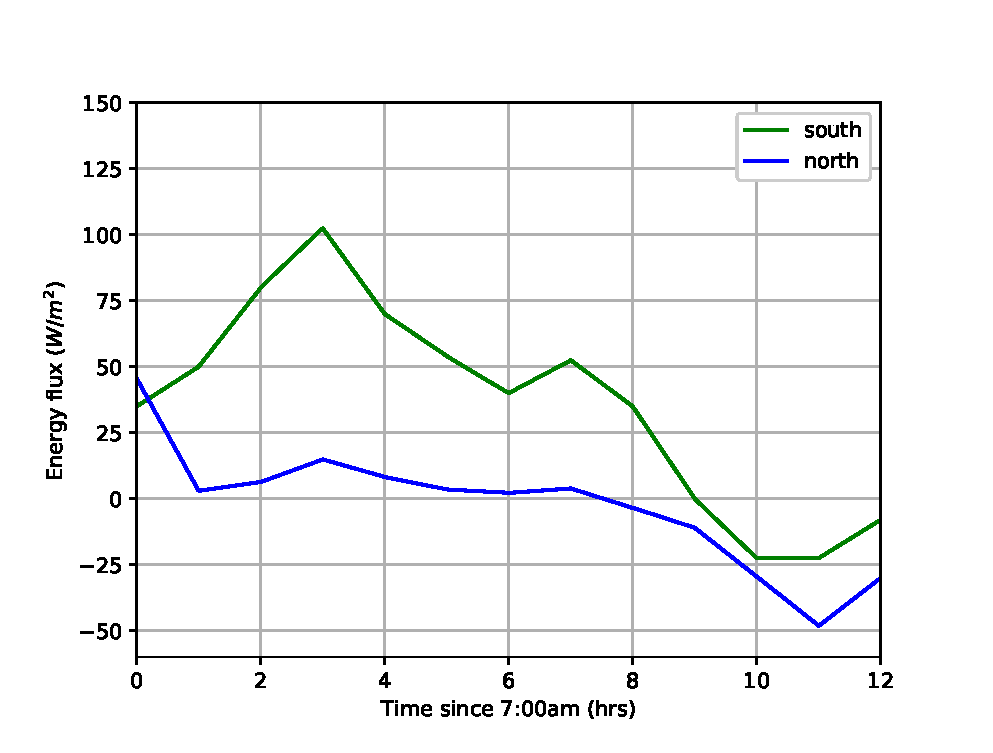
\includegraphics[width=1\linewidth]{fig/combinedHeatSource.eps}
%  \caption{Linear combination of the source terms, $H + (1-\alpha)(S_{dir}+S_{dif})+(IR_{in}-IR_{out})$ on the north and south sides of the tree. Source: \ref{potter_andresen}} % fig. 4 in source
%  \label{fig:combined_source_term}
%\end{figure}

Figure \ref{fig:combined_source_term} shows the linear combination of the source terms $H + (1-\alpha)(S_{dir}+S_{dif})+(IR_{in}-IR_{out})$ on the north and south sides of the tree from \ref{potter_andresen}. 
Due to the COVID-19 pandemic, our hardware team was not able to collect these data in the local forest. We therefore use the aspen simulations data found in \ref{potter_andresen}. One of the future aspect of this work is to collect experimental data locally, and run our numerical simulation again.

\section{Finite difference (FD) schemes for the heat equations}
We compute the temperature distribution in tree trunks numerically with the Finite difference method, as it is simple to implement, and robust \ref{2017book}. Here in particular, we discretize the continuous equation in one dimension using the Crank-Nicolson scheme, due to its advantage in stability, and higher accuracy in time \ref{leveque}. %For the two dimension problem, we apply the standard forward in time, central difference in space.
%\subsection{1D scheme}
%There are approximately 12 inches between the exterior of the tree and the core of the tree (on moderately sized trees such as the ponderosa pine in the forests that we study). 
The radius of the tree stem is approximately 12 inches between the exterior and core in moderately sized trees we target for our study. The aluminum rod (Fig.\ref{fig:rod}) in our TEG hardware system  is about 12 inches in length with a 0.5 inch radius, embedded in the trunk of a tree at approximately breast height. Due to the size comparisons of our devices and the tree trunk, it is more appropriate to model the heat equation in polar form \eqref{heat1d} than the standard Cartesian form. Let $T^n_{i} \approx T(r_i,t_n)$ denote the numerical solution at the point $(r_i,t_n)$, $\Delta t$ the time step, and $\Delta r$ grid size. 
With second order central difference in space 
\begin{equation}\frac{\partial T}{\partial r}\approx\frac{T_{i+1}-T_{i-1}}{2\Delta r}\end{equation}
\begin{equation}\frac{\partial^2 T}{\partial r^2}\approx\frac{T_{i-1}-2T_{i}+T_{i+1}}{(\Delta r)^2}\end{equation}
and first order forward in time
\begin{equation}\frac{\partial T}{\partial t}\approx\frac{T^1-T^0}{\Delta t},\end{equation}
we obtain the Crank-Nicolson method by averaging the above spatial differences in time:
\begin{align}
&(T^{n+1}_i - T^n_i)/\Delta t = 1/(4ar_i\Delta r)(T^n_{i+1}-T^n_{i-1} + T^{n+1}_{i+1}-T^{n+1}_{i-1} )\nonumber\\
&+1/(2a(\Delta r)^2)(T^n_{i-1} - 2T^n_i + T^n_{i+1} + T^{n+1}_{i-1} - 2T^{n+1}_i + T^{n+1}_{i+1}),\label{1dCNscheme}
\end{align}
where $a = \frac{\rho c}{k}$.

We implement boundary conditions in the numerical scheme. For the boundary at the center of the tree, we follow the same no-flux Neumann condition in \ref{firestem2d}. We use the second order central difference approximation at $r=0$: 
\begin{equation}
    \frac{\partial T}{\partial r}\bigg|_{r=0}\approx \frac{T_2-T_0}{2\Delta r}=0.
\end{equation} % should try with Dirichlet conditions as well, if more info of temperature is known. Our original modeling still makes sense: center temperature is const + small oscillation.
Equation \eqref{1dCNscheme} gives a representation for the ghost cell value $T_0$ in terms of $T_2$, which is implemented in the first row of the matrix below. 

For the outer boundary condition at the surface of the tree, we implement the Dirichlet condition with ambient temperature $g_1(t)$
\begin{equation}
    T(r,t)\bigg|_{surface}=g_1(t),
\end{equation}
in the last row of the following matrix equation. The source term is also present in the last row of the following matrix equation.

Together, we solve the following system to compute the heat distribution in the tree trunk: % ref: a primer to PDEs, Salsa et al
\begin{equation*}
    \left( \begin{array}{cccc}
1+\beta & -\beta & & 0\\
\alpha_2 & 1+\beta & -\gamma_2 & \\
\ddots& \ddots & \ddots  & \\
& \alpha_{m-1} & 1+\beta & -\gamma_{m-1} \\
0 & & \alpha_m & 1+\beta \end{array} \right)\left(\begin{array}{c}
     T^1_1  \\
     T^1_2 \\
     \vdots\\
     T^1_{m-1}\\
     T^1_m
\end{array}\right)=\end{equation*}
\begin{equation}
  \left(\begin{array}{c}
     (1-\beta)T^0_1+\beta T^0_2  \\
  -\alpha_2T^0_1+(1-\beta) T^0_2+\gamma_2T^0_3 \\
     \vdots\\
    -\alpha_{m-1}T^0_{m-2} +(1-\beta)T^0_{m-1}+\gamma_{m-1}T^0_m\\
    -\alpha_{m}T^0_{m-1} +(1-\beta) T^0_m +\gamma_m(g_1(t)+g_1(t+\Delta t))+source
\end{array}\right), 
\end{equation}
%\begin{equation}\left( \begin{array}{cccc}
%1-\beta & \beta & & 0\\
%-\alpha_2 & 1-\beta & \gamma_2 & \\
%\ddots& \ddots & \ddots  & \\
%& -\alpha_{m-1} & 1-\beta & \gamma_{m-1} \\
%0 & & -\alpha_m & 1-\beta \end{array} \right)\left(\begin{array}{c}
%     T^0_1  \\
%     T^0_2 \\
%     \vdots\\
%     T^0_{m-1}\\
%     T^0_m
%\end{array}\right)+\left(\begin{array}{c}
%     0  \\
%     0 \\
%     \vdots\\
%     0\\
%     r_m(g_1(t)+g_1(t+Delta t))
%\end{array}\right)
%\end{equation}
where $\alpha_i = \frac{\Delta t}{4ar_i\Delta t}-\frac{\Delta t}{2a(\Delta r)^2}$, $\beta = \frac{\Delta t}{a(\Delta r)^2}$, and $\gamma_i = \frac{\Delta t}{4ar_i\Delta t}+\frac{\Delta t}{2a(\Delta r)^2}$. %\textcolor{red}{Update by Yajun: code based on the above discretization is fixed, on github/yan, code is called \tt{heat1D\_CNpolar\_forPaper.py}}

% \section{2D scheme}
% Here we consider temperature that depends on time $t$, radial location $r$, and angular location $\phi$. We denote the numerical approximation to $T(r,\phi,t)$ by $T(r,\phi,t)\approx T^0_{i,j}$, where the new index $j$ denotes the index for angle $\phi$. 

% \begin{align}
% T^1_{i,j}=& \frac{k\Delta t}{\rho c}\bigg[\underbrace{\frac{1}{(\Delta r)^2}\bigg(T^0_{i-1,j}+T^0_{i+1,j}-2T^0_{i,j}\bigg)}_{\frac{\partial^2T}{\partial r^2}}+\nonumber\\
% &\underbrace{\frac{1}{2r_i\Delta r}\bigg(T^0_{i+1,j}-T^0_{i-1,j}\bigg)}_{\frac{1}{r}\frac{\partial T}{\partial r}}\nonumber\\
% +& \underbrace{\frac{1}{r_i^2(\Delta \phi)^2}\bigg(T^0_{i,j-1}+T^0_{i,j+1}-2T^0_{i,j}\bigg)}_{\frac{1}{r^2}\frac{\partial^2 T}{\partial \phi^2}}\bigg]+T^0_{i,j},
% \end{align}
% with $k_1= \frac{k\Delta t}{\rho c(\Delta r)^2}$, $k_2 = \frac{k\Delta t}{2\rho cr_i\Delta r}$, and $k_3= \frac{k\Delta t}{\rho cr_i^2(\Delta \phi)^2}$, above equation can be implemented as
% \begin{align}
% &T^1_{i,j}= k_1\bigg(T^0_{i-1,j}+T^0_{i+1,j}-2T^0_{i,j}\bigg)+k_2\bigg(T^0_{i+1,j}-T^0_{i-1,j}\bigg)\nonumber\\
% &+k_3\bigg(T^0_{i,j-1}+T^0_{i,j+1}-2T^0_{i,j}\bigg)+T^0_{i,j},
% \end{align}
% where we obtain $T^1_{i,j}$ each time step with $T$ values in several locations from previous step. This system of equations can be solved directly.


\section{Numerical experiments and discussion of results}
With the above FD scheme, combined example source term, and a constant temperature at 7 am as initial condition, we obtain the following figures of temperature distributions.
% \begin{figure}
%      \centering
%      \begin{subfigure}[b]{0.5\textwidth}
%          \centering
%          \includegraphics[width=\textwidth]{fig/tempN38new1.eps}
%          \caption{Temperature distribution throughout the day, north aspect}
%          \label{fig:tempN38}
%      \end{subfigure}
%      \hfill
%      \begin{subfigure}[b]{0.5\textwidth}
%          \centering
%          \includegraphics[width=\textwidth]{fig/tempS38new1.eps}
%          \caption{Temperature distribution throughout the day, south aspect}
%          \label{fig:tempS38}
%      \end{subfigure}
%         \caption{For a tree with 12 inch radius, temperature distribution in the north and south aspects, with depth of about 9 inches.}
%         \label{fig:at38}
% \end{figure}
\begin{comment}
\begin{figure}
  \includegraphics[width=1\linewidth]{fig/temp38.png}
  \caption{For a tree with 12 inch radius, temperature distribution in the north and south aspects, with depth of about 9 inches.} 
  \label{fig:at38}
\end{figure}
\end{comment}

% \begin{figure}
%      \centering
%      \begin{subfigure}[b]{0.5\textwidth}
%         \centering
%          \includegraphics[width=\textwidth]{fig/tempN29new1.eps}
%          \caption{Temperature distribution throughout the day, north aspect}
%          \label{fig:tempN29}
%      \end{subfigure}
%     \hfill
%      \begin{subfigure}[b]{0.5\textwidth}
%         \centering
%         \includegraphics[width=\textwidth]{fig/tempS29new1.eps}
%          \caption{Temperature distribution throughout the day, south aspect}
%          \label{fig:tempS29}
%      \end{subfigure}
%        \caption{For a tree with 12 inch radius, temperature distribution in the north and south aspects, with depth about 7 inches.}
%         \label{fig:at29}
% \end{figure}
 
\begin{comment}
  \begin{figure}
  \includegraphics[width=1\linewidth]{fig/temp29.png}
  \caption{For a tree with 12 inch radius, temperature distribution in the north and south aspects, with depth of about 7 inches.} 
  \label{fig:at29}
\end{figure}
\end{comment}


% \begin{figure}
%      \centering
%      \begin{subfigure}[b]{0.5\textwidth}
%          \centering
%          \includegraphics[width=\textwidth]{fig/tempN2new1.eps}
%          \caption{Temperature distribution throughout the day, north aspect}
%          \label{fig:tempN2}
%      \end{subfigure}
%      \hfill
%      \begin{subfigure}[b]{0.5\textwidth}%          \centering
%          \includegraphics[width=\textwidth]{fig/tempS2new1.eps}
%          \caption{Temperature distribution throughout the day, south aspect}
%          \label{fig:tempS2}
%      \end{subfigure}
%        \caption{For a tree with 12 inch radius, temperature distribution in the north and south aspects, near tree center.}
%         \label{fig:at2}
% \end{figure}

\begin{comment}\begin{figure}
  \includegraphics[width=1\linewidth]{fig/temp2.png}
  \caption{For a tree with 12 inch radius, temperature distribution in the north and south aspects, near tree center.} 
  \label{fig:at2}
\end{figure}
\end{comment}

From Fig.\ref{fig:at38}, Fig.\ref{fig:at29}, and Fig.\ref{fig:at2}, we conclude that the south aspects uniformly have a larger temperature range throughout the day; therefore it is preferable to install all TEG devices in the south. We also see that, the further away we are from the tree center, the trend of temperature is more consistent with heat flux. From our simulations, temperature distributions with medium depth don't differ significantly, for example, temperature measured at depth 7 to 9 inches have similar temperature ranges. We expected fairly constant temperature near the center of the trunk, but our simulation does not reflect that, and this is another issue we expect to address in our future work.
With measurements of the tree surface temperature, our hardware team can adjust the length of the rod for optimal voltage generated from the temperature differences. The highest temperatures uniformly occur roughly 8 or 9 hours after we start the measurements, with lowest temperature in the beginning and end of the measurement cycle. 

The simulation appears to be excessively warm overall for the north aspect; this is due to the limitation of the example data as described in \ref{potter_andresen}, and our interpretation of the example data. %\textcolor{red}{Is there a specific shortcoming of the example dataset that we can state here? Yes- too warm overall. Does that mean the temperature is unrealistically large? Or too warm for the purpose of the TEGs?- Too warm in general in their temperature simulation. I don't think we know what the TEG needs. Here is from Potter and Andresen: The aspen simulation appears to have been too warm, overall. 

\section{Conclusion and on-going work}
In this work, we modeled the temperature distribution in a tree trunk with the one dimensional heat equation in cylindrical coordinates, with various heat sources. We simplified the model to fit our purpose of studying the temperature distribution for applying TEG devices efficiently \ref{thermoelectric}. We applied a Crank-Nicolson FD scheme for numerical simulation, with example data, and analyzed the optimal aspect for installation of devices, as well as depth of installation. 

We are working on higher dimension simulations for the temperature distribution for tree trunks, to gain more insight for other potential installation aspects. We will also be running these simulations locally once we have access to more data specific to tree species in western Washington State, as well as data from our collaborators in Brazil in Azores.

\section*{Acknowledgment}
We appreciate the contribution to this work by Nick Purcell of the University of Washington (data collection), and Professor Cleonilson Protasio de Souza of the University of Paraiba.


\section*{References}
\begin{enumerate}[label={[\arabic*]}]

\item B. R. Helliker and S. L. Richter, “Subtropical to boreal convergence of tree-leaf temperatures,” Nature, vol. 454, July 2008. [Online.] Available: Academic OneFile, http://find.galegroup.com. [Accessed July 21, 2020]. \label{treeleaf}

\item P. Souza, F. Carvalho, F. Silva, H. Andrade, N. Silva, O. Baiocchi, and I. Müller, “On Harvesting Energy from Tree Trunks for Environmental Monitoring,” International Journal of Distributed Sensor Networks, pp. 1-9, 2016. \label{souza}

\item B. E. Potter and J. A. Andresen, “A Finite-Difference Model of Temperatures and Heat Flow within a Tree Stem,” Canadian Journal of Forest Research, vol. 32, no. 3, pp. 548–555, 2002.\label{potter_andresen}

\item  E. K. Chatziefstratiou, et al., “FireStem2D – A Two-Dimensional Heat Transfer Model for Simulating Tree Stem Injury in Fires,” PLoS ONE, vol. 8, no. 7, p.e70110, July 2013.\label{firestem2d}

\item W. Simpson, A. TenWolde, “Physical properties and moisture relations of wood,” in \textit{ Wood handbook: wood as an engineering material}, Madison, WL: USDA Forest Service, Forest Products Laboratory, 1999, General technical report FPL, GTR-113: pp. 3.1-3.24\label{parameter} 

\item S. Linge, H. P. Langtangen, “Diffusion Equations,” in \textit{Finite Difference Computing with PDEs}, vol. 6, 1st ed. Springer, 2017, ch.3, pp. 207-322.\label{2017book}

\item R. J. LeVeque, \textit{ Finite difference methods for ordinary and partial differential equations}, SIAM, 2007\label{leveque} 

\item D. Yan, F. P. Dawson, M. Pugh, and A. A. El-Deib, “Time-Dependent Finite-Volume Model of Thermoelectric Devices,” IEEE Transactions on Industry Applications, vol. 50, no. 1, pp. 600-608, 2014.\label{thermoelectric}

\item Y. An, O. Baiocchi, M. Hockman, and S. Teng, "Computational model for temperature in tree trunk for energy harvesting," 2020 IEEE International IOT, Electronics and Mechatronics Conference (IEMTRONICS), Vancouver, BC, Canada, 2020, pp. 1-6, 

doi: 10.1109/IEMTRONICS51293.2020.9216373.\label{1Dtree}

% The following sources are not cited in text (yet)

% \item W. Bownman, “Sapwood temperature gradients between lower stems and the crown do not influence estimates of stand-level stem CO2 efflux,” Tree Physiology, vol. 28, no. 10, pp. 1553-1559, August 2008. [Online]. Available: https://academic.oup.com/treephys/article/28/10/1553/1647174. [Accessed July 21, 2020].\label{sapwood}

% \item J. Chen, J. F. Franklin, T. A. Spies, “An empirical model for predicting diurnal air-temperature gradients from edge into old-growth Douglas-fir forest,” Ecological Modeling, vol. 67, no. 2, pp. 179-198, 1993.\label{airtempforest}

% \item S. Tanja, et al., “Air temperature triggers the recovery of evergreen boreal forest photosynthesis in spring,” Global Change Biology, vol. 9, pp. 1410-1426, 2003.\label{evergreen}

 


\end{enumerate}

% \section*{References}
% Please number citations consecutively within brackets \cite{IEEEhowto:IEEEtranpage}. The 
% sentence punctuation follows the bracket \cite{b2}. Refer simply to the reference 
% number, as in \cite{b3}---do not use ``Ref. \cite{b3}'' or ``reference \cite{b3}'' except at 
% the beginning of a sentence: ``Reference \cite{b3} was the first $\ldots$''

% Number footnotes separately in superscripts. Place the actual footnote at 
% the bottom of the column in which it was cited. Do not put footnotes in the 
% abstract or reference list. Use letters for table footnotes.

% Unless there are six authors or more give all authors' names; do not use 
% ``et al.''. Papers that have not been published, even if they have been 
% submitted for publication, should be cited as ``unpublished'' \cite{b4}. Papers 
% that have been accepted for publication should be cited as ``in press'' \cite{b5}. 
% Capitalize only the first word in a paper title, except for proper nouns and 
% element symbols.

% For papers published in translation journals, please give the English 
% citation first, followed by the original foreign-language citation \cite{b6}.

% \bibliographystyle{./bibliography/IEEEtran}
% \bibliography{./bibliography/IEEEabrv,./bibliography/IEEEexample}

% \vspace{12pt}
% \color{red}
% IEEE conference templates contain guidance text for composing and formatting conference papers. Please ensure that all template text is removed from your conference paper prior to submission to the conference. Failure to remove the template text from your paper may result in your paper not being published.

\end{document}
